% !TEX TS-program = pdflatexmk
\documentclass{article}
\usepackage[latin1]{inputenc} 

\title{Figure code for Pedersen et al. (2013), Nature Biotechnology}
\author{Lykke Pedersen, Peter H Hagedorn, Marie Lindholm and Morten Lindow}


\usepackage{Sweave}
\begin{document}
\Sconcordance{concordance:Vignette2.tex:Vignette2.Rnw:%
1 33 1 1 0 6 1 1 2 1 0 1 2 4 0 1 2 3 1 1 3 2 0 1 2 1 0 1 1 3 0 2 2 4 0 %
2 2 1 0 1 2 1 0 1 2 1 1 1 3 1 0 1 6 5 0 1 1 1 2 1 0 3 1 1 3 2 0 1 3 2 0 %
1 3 2 0 1 3 2 0 1 3 5 0 1 2 8 1 1 2 1 0 1 3 2 0 2 1 1 2 1 0 2 1 3 0 1 2 %
9 1 1 2 1 0 1 1 3 0 2 2 1 0 2 1 3 0 2 2 1 0 1 2 1 0 2 1 1 2 1 0 1 1 3 0 %
1 2 8 1 1 2 1 0 3 1 1 3 1 0 1 1 2 2 1 3 2 0 1 2 6 1 1 2 1 0 2 1 3 0 1 2 %
7 1 1 3 2 0 1 1 1 2 1 1 1 2 1 0 1 2 1 0 1 2 1 3 2 0 5 1 1 2 1 0 2 1 3 0 %
1 2 7 1 1 3 2 0 1 1 3 2 1 0 1 1 1 2 7 1 1 2 1 0 2 1 3 0 1 2 77 1}



\maketitle
With the gain of increasing reproducibility, this vignette includes the commands to produce Fig. 2 from ``A kinetic model of enzyme recruiting oligonucleotides predicts an optimal affinity and thus explains why shorter and less affine oligonucleotides may be more potent". The functions from the ASOmodels are used and the package is loaded by the commands

\begin{Schunk}
\begin{Sinput}
> require(devtools)
> system('R CMD install ~/Documents/ASOmodels/ASOmodels')
> require(ASOmodels)
\end{Sinput}
\end{Schunk}

\section*{Kinetic model figures}
\subsection*{Figure 2a}
Parameters for the ASO model:
\begin{Schunk}
\begin{Sinput}
> parms <- c(Et = 1,KdOT = 0.3,kOpT = 0.2,KdOTE = 70,kOTpE = 5,  
+            vprod = 0.2,vdegrad = 0.04,alpha=0.1,kcleav = 8)
\end{Sinput}
\end{Schunk}
The initial concentrations:
\begin{Schunk}
\begin{Sinput}
> init <- c(T=parms['vdegrad']/parms['vdegrad'], OT=0, OTE=0, 
+           E=parms['Et'], O=100, OCE=0, OC=0)
\end{Sinput}
\end{Schunk}
Timesteps for which the simulation is performed:
\begin{Schunk}
\begin{Sinput}
> TimeSteps <- c(seq(0,4.3,by=5E-2),seq(5,65,by=1))
\end{Sinput}
\end{Schunk}
Using \texttt{vode()} the ASO model is simulated in time.
\begin{Schunk}
\begin{Sinput}
> solASO <- vode(init,TimeSteps,diffASO,parms)
\end{Sinput}
\end{Schunk}
The timetraces for the concentrations of $[O]$, $[T]$, $[OT]$, $[OTE]$, and $[E]$ are plotted:
\begin{Schunk}
\begin{Sinput}
> SSvalue <- signif(last(solASO)[-1],2)
> solASO <- apply(solASO[,2:8],2,
+                 function(x) (x-min(x))/max(x-min(x)) )
> colVAR <- c('black','darkgreen','darkred','orange','green')
> xtime <- TimeSteps <= 35
> par(mar=c(3.2,3.4,0.1,0.1),bty='n',mgp=c(2,0.7,0),cex=0.6,cex.axis=1,las=1)
> for(i in 1:5){ 
+   if(i!=1) par(new=TRUE)
+   plot(TimeSteps[xtime], solASO[xtime,i], yaxt='n', xaxt='n',
+        ylab='relative concentrations', xlab='minutes',
+        las=1, col=colVAR[i], type='l', ylim=c(0,1), xlim=c(0,35+26))
+ }
> xtime <- 40
> for(i in 1:5) lines(xtime+0:20,rep(last(solASO)[i],21),
+                     col=colVAR[i])
> axis(1,at=c((0:3)*10,45),label=c((0:3)*10,''))
> axis(1,at=45,label='steady-\nstate',mgp=c(0,1.6,0))
> axis(2,at=c(0,1),label=c('min','max'),las=1)
> #O
> text(xtime,last(solASO)[5]-0.05,col=colVAR[5],adj=0,
+      substitute(O == e~nM,list(e=SSvalue[5])))
> #T
> text(xtime,0.05,col=colVAR[1],adj=0,
+      substitute(T == e*pM,list(e=1e3*SSvalue[1])))
> #OT
> text(xtime,last(solASO)[2]-0.05,col=colVAR[2],adj=0,
+      substitute(OT== e*nM,list(e=SSvalue[2])))
> #OTE
> text(xtime,last(solASO)[3]+0.05,col=colVAR[3],adj=0,
+      substitute(OTE == e*pM,list(e=1e3*SSvalue[3])))
> #E
> text(xtime,last(solASO)[4]+0.05,col=colVAR[4],adj=0,
+      substitute(E == e*nM,list(e=SSvalue[4])))
\end{Sinput}
\end{Schunk}
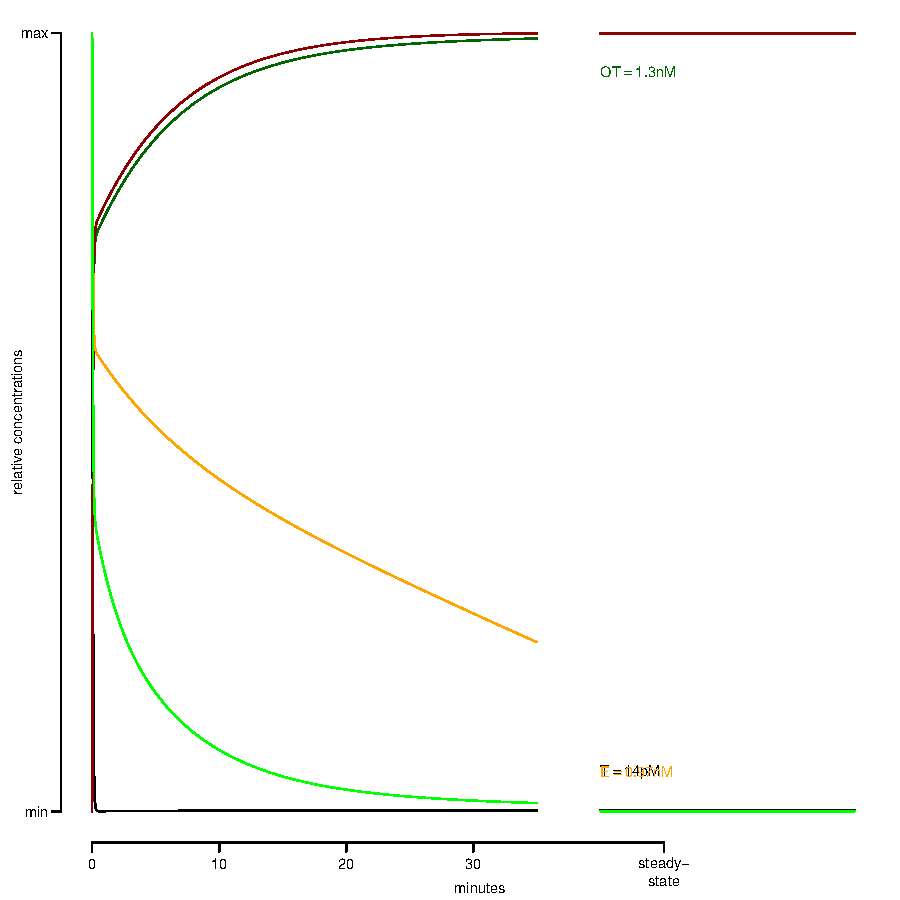
\includegraphics{Vignette2-006}

\subsection*{Figure 2b}
\begin{Schunk}
\begin{Sinput}
> curve(Trel.function,1E-3,5E2,log='x', lwd=2,ylim=c(0,1),
+       ylab=expression(T[rel]),xaxt='n',
+       xlab='Total oligonucleotide conc (nM)')
> abline(h=Trel.function(1E9),lty=2)
> abline(v=IC50(parms['KdOT']),lty=2)
> axis(1,at=10^c(-3,-1,1,3),
+      labels=pretty10expLP(10^c(-3,-1,1,3),drop.1=T))
> axis(1,at=IC50(parms['KdOT']),label=expression(IC[50]))
> axis(2,at=Trel.function(1E6),
+      label=expression(T[rel*','*min]),las=1)
\end{Sinput}
\end{Schunk}
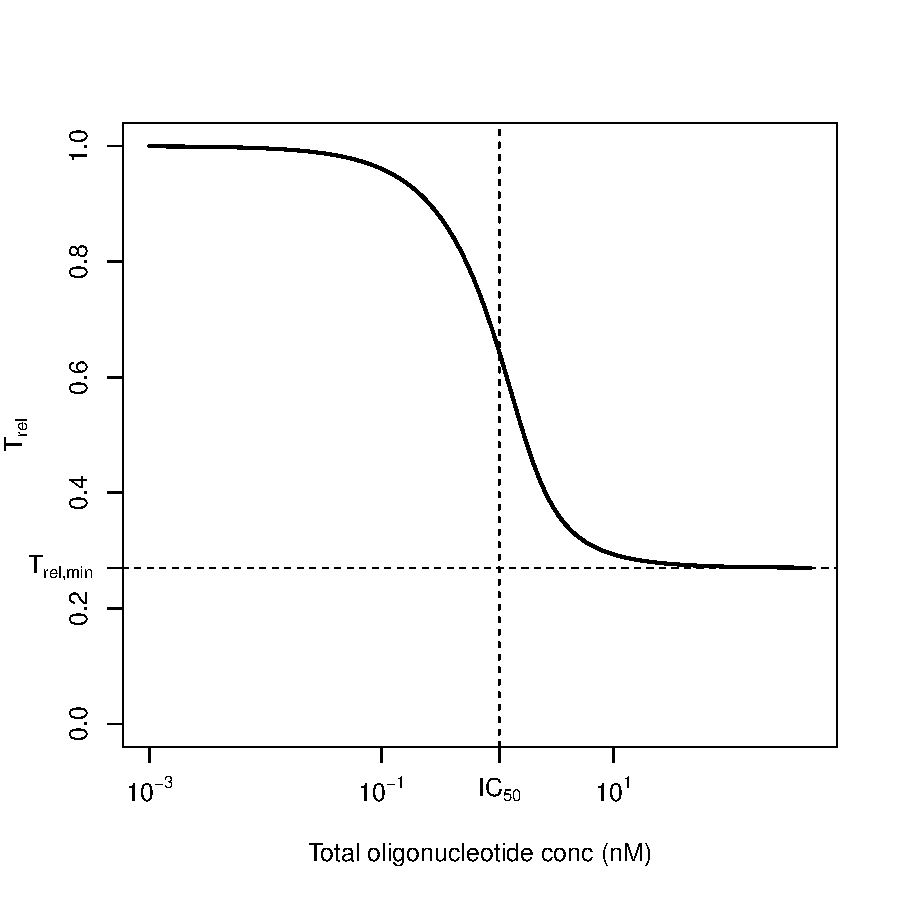
\includegraphics{Vignette2-007}

\subsection*{Figure 2c}
\begin{Schunk}
\begin{Sinput}
> D1_seq <- 10^seq(-3,3.2,by=0.25)
> ICfit <- sapply(D1_seq,IC50)
> parmsNO <- c(parms,k3=parms['kOpT']*parms['KdOT']/parms['alpha'])
> names(parmsNO)[length(parmsNO)] <- 'k3'
> ICfitNO <- sapply(D1_seq,IC50NO)
> plot(D1_seq,ICfit,log='xy',yaxt='n',type='l',xaxt='n',
+      xlab=expression(D[OT]~'(nM)'),ylab=expression(IC[50]~'(nM)'))
> lines(D1_seq,ICfitNO,lty=2)
> axis(2,at=c(2,20,200),labels=c(2,20,200))
> axis(1,at=10^pretty(log10(D1_seq)),
+      labels=pretty10expLP(10^pretty(log10(D1_seq)),drop.1=T),)
> legend('topleft',c('Coupling','No coupling'),lty=c(1,2),bty='n')
\end{Sinput}
\end{Schunk}
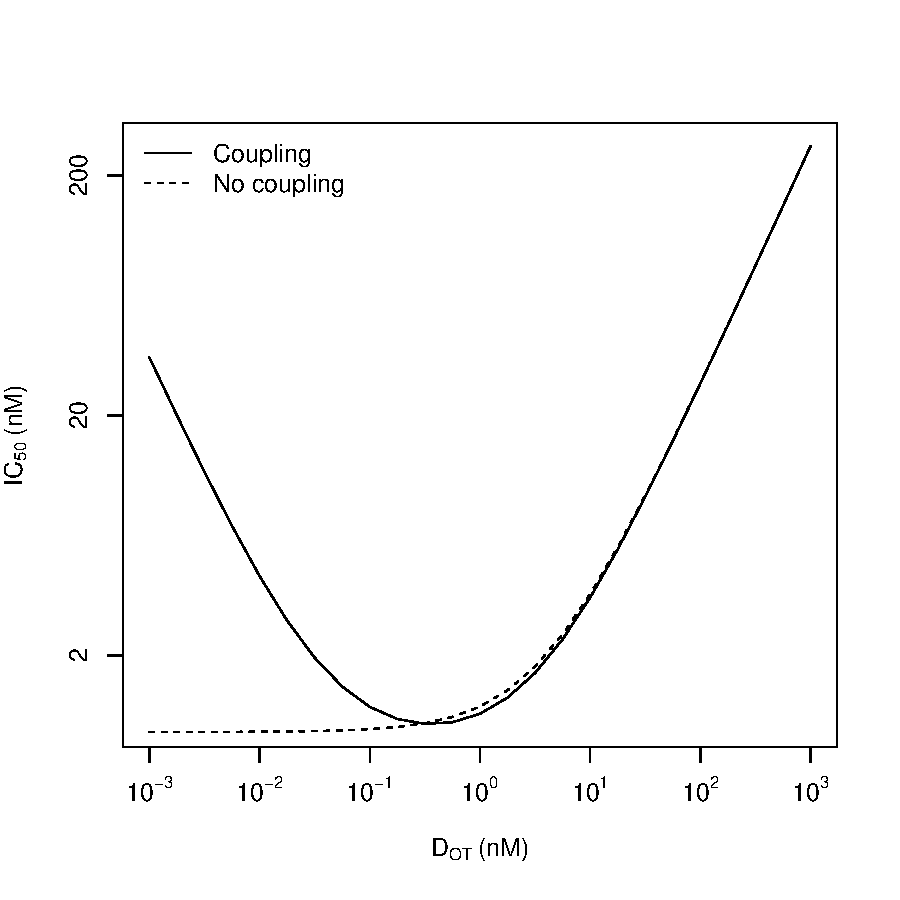
\includegraphics{Vignette2-008}

\section*{Experimental data figures}
\section*{Figure 2d}
\begin{Schunk}
\begin{Sinput}
> dat <- read.table('../vignettes/SuppFile2.txt',
+                   header=T,sep='\t')
> colL <- c('red','orange','darkgreen','','darkblue','','purple','','black')
> ### Frieden et al, 2003
> dat.F <- dat[dat$Study=="Frieden 2003",]
> cohigh.F <- 63; colow.F <- 53
> tmp <- abs(cohigh.F-colow.F)
> cut.F <- cut(dat.F$Predicted.Tm,c(0,colow.F,cohigh.F,100),labels=F)
> Fx <- lapply(1:3,function(i)dat.F$Predicted.Tm[cut.F==i])
> Fy <- lapply(1:3,function(i) dat.F$Dose.2nm[cut.F==i])
> Flength <- dat.F$Oligo.length
> bp <- barplot(sapply(Fy,mean),ylim=c(0,55), las=1, axes=F,
+               yaxs='i',xaxs='i',space=0.01)
> plotCI(bp[,1],sapply(Fy,mean),sapply(Fy,sd),
+        add=T,pch=NA, gap=0,yaxs='i')
> par(new=T)
> plot(unlist(Fx),unlist(Fy),xlim=c(colow.F-tmp,cohigh.F+tmp),
+      ylim=c(0,55), pch=19, col=colL[Flength-11],xaxt='n',
+      ylab='% target measured from luciferase',
+      xlab=expression(T[m]~'('*degree*C*')'),yaxs='i',xaxs='i')
> axis(1,at=c(colow.F,cohigh.F),labels=as.character(c(colow.F,cohigh.F)))
> legend('bottomright',as.character(sort(unique(Flength))),
+        pch=19, col=colL[sort(unique(Flength))-11],bg='white')
\end{Sinput}
\end{Schunk}
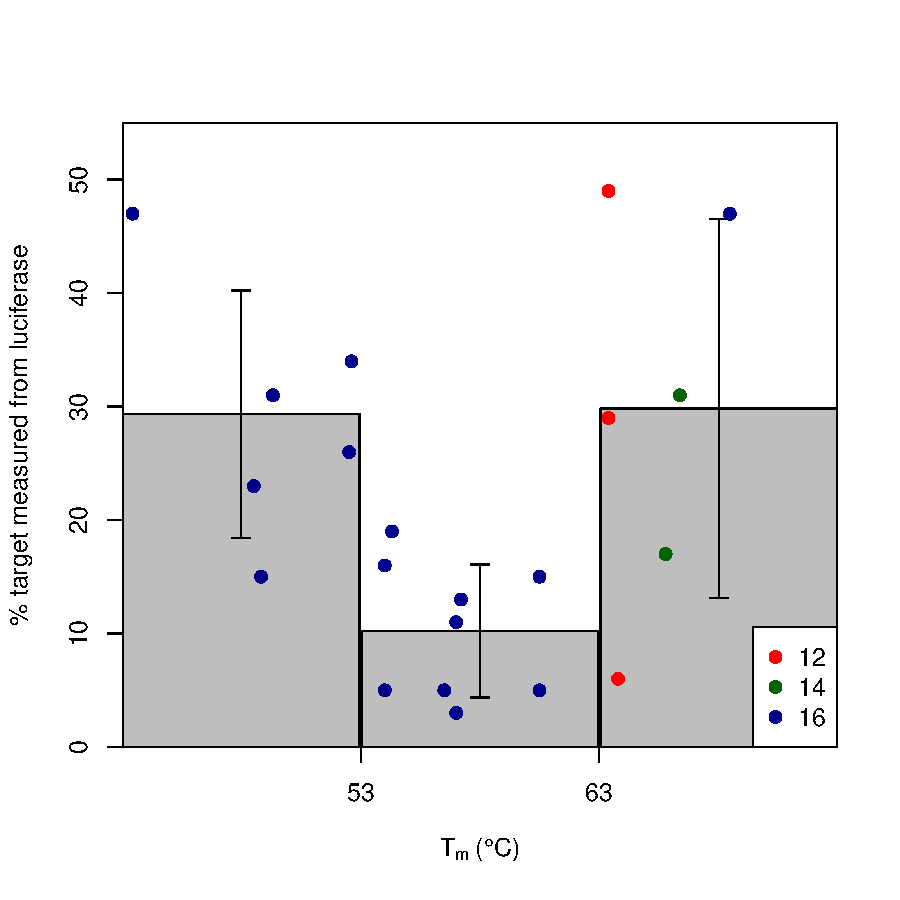
\includegraphics{Vignette2-009}

\section*{Figure 2e}
\begin{Schunk}
\begin{Sinput}
> ### Stanton et al 2012
> dat.S <- dat[dat[,1]=="Stanton 2012",]
> cohigh.S <- 61; colow.S <- 46
> tmp <- abs(cohigh.S-colow.S)
> cut.S <- cut(dat.S$Predicted.Tm,c(0,colow.S,cohigh.S,100),labels=F)
> Sx <- lapply(1:3,function(i)dat.S$Predicted.Tm[cut.S==i])
> Sy <- lapply(1:3,function(i) dat.S$Dose.3nm[cut.S==i])
> Slength <- dat.S$Oligo.length
> bp <- barplot(sapply(Sy,mean),ylim=c(0,105), las=1,axes=F,
+               yaxs='i', xaxs='i',space=0.01)
> plotCI(bp[,1],sapply(Sy,mean),sapply(Sy,sd),add=T,pch=NA, gap=0,yaxs='i')
> par(new=T)
> plot(unlist(Sx),unlist(Sy),xlim=c(colow.S-tmp,cohigh.S+tmp),
+      ylim=c(0,105), pch=19,col=colL[Slength-11],xaxt='n',
+      ylab='% target measured from PCR',
+      xlab=expression(T[m]~'('*degree*C*')'),yaxs='i',xaxs='i')
> axis(1,at=c(colow.S,cohigh.S),labels=as.character(c(colow.S,cohigh.S)))
> legend('bottomright',as.character(sort(unique(Slength))),
+        pch=19,col=colL[sort(unique(Slength))-11],bg='white')
\end{Sinput}
\end{Schunk}
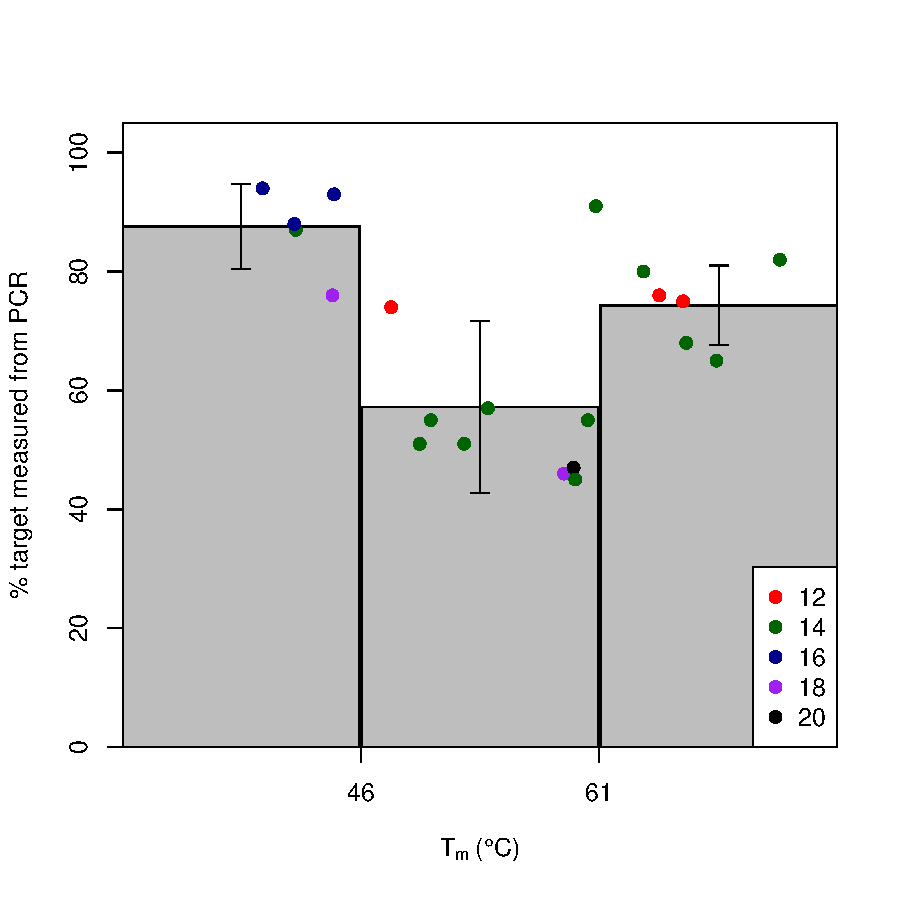
\includegraphics{Vignette2-010}
\section*{Figure 2f}
\begin{Schunk}
\begin{Sinput}
> ### Pedersen et al, 2013
> dat.P <- dat[dat$Study=="Pedersen 2013",]
> cohigh.P <- 56; colow.P <- 47
> tmp <- abs(cohigh.P-colow.P)
> cut.P <- cut(dat.P$Predicted.Tm,c(0,colow.P,cohigh.P,100),labels=F)
> Px <- lapply(1:3,function(i)dat.P$Predicted.Tm[cut.P==i])
> Py <- lapply(1:3,function(i) dat.P$IC50[cut.P==i])
> Plength <- dat.P$Oligo.length
> bp <- barplot(sapply(Py,mean),ylim=c(0,0.016), las=1,
+               axes=F,yaxs='i', xaxs='i',space=0.01)
> plotCI(bp[,1],sapply(Py,mean),sapply(Py,sd),add=T,
+        pch=NA, gap=0,yaxs='i')
> par(new=T)
> plot(unlist(Px),unlist(Py),xlim=c(colow.P-tmp,cohigh.P+tmp),ylim=c(0,0.016), 
+      pch=19,col=colL[Plength-11],xaxt='n',ylab=expression(IC[50]~'('*nM*')'),
+      xlab=expression(T[m]~'('*degree*C*')'),yaxs='i',xaxs='i')
> axis(1,at=c(colow.P,cohigh.P),labels=as.character(c(colow.P,cohigh.P)))
> legend('bottomright',as.character(sort(unique(Plength))),
+        pch=19,col=colL[sort(unique(Plength))-11],bg='white')
\end{Sinput}
\end{Schunk}
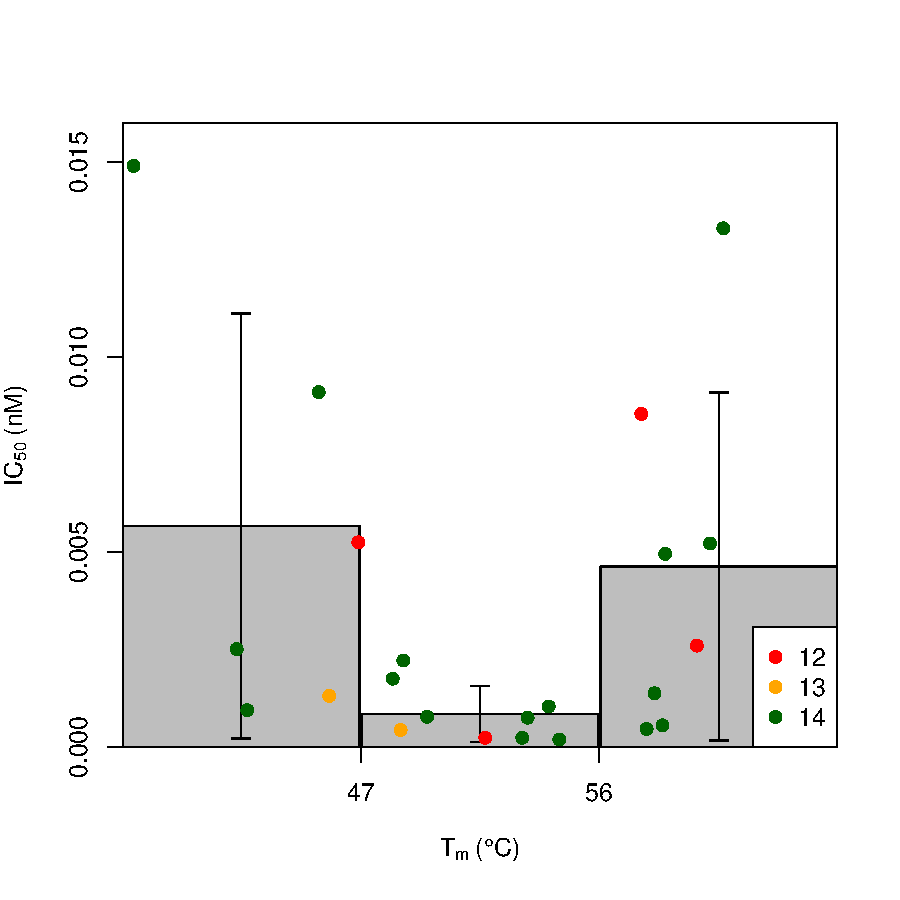
\includegraphics{Vignette2-011}


%pdf('PCH.pdf',width=3,height=3)
%par(mar=c(4,4,1,1))
%plot(unique(c(al,bl,cl)),pch=unique(c(al,bl,cl))-11,ylim=c(12,21),
%     panel.first=grid(),xaxt='n',xlab=NA,ylab='oligonucleotide length')


\end{document}
